\documentclass[english]{article}
\usepackage[T1]{fontenc}
%\usepackage[latin1]{inputenc}
\usepackage{enumerate}
\usepackage{setspace}
\usepackage{amsmath,amssymb,amsthm}
\usepackage{graphicx}
\usepackage[round]{natbib}
\usepackage[nohead]{geometry}
\usepackage[bottom]{footmisc}
\usepackage{indentfirst}
\usepackage{endnotes}
\usepackage{graphicx}%
\usepackage{eurosym}
\usepackage{array}
\usepackage{booktabs}
\usepackage[section]{placeins} % keep tables within their section
\makeatletter
\AtBeginDocument{%
  \expandafter\renewcommand\expandafter\subsection\expandafter{%
    \expandafter\@fb@secFB\subsection
  }%
}
\makeatother
\usepackage{siunitx}
\usepackage{dcolumn}
\newcolumntype{.}{D{.}{.}{-1}}
\usepackage{caption}
\usepackage{subcaption}
\usepackage{tabularx}
\usepackage[flushleft]{threeparttable}
% \usepackage[hidelinks]{hyperref}
\usepackage{floatrow} %[capposition=top]
\usepackage{bbm}
\interfootnotelinepenalty=10000
\floatsetup{footposition=bottom,capposition=top}
\renewcommand{\labelitemi}{--}
\renewcommand{\labelitemii}{$\bullet$}
\bibliographystyle{chicago}
% \geometry{left=1in,right=1in,top=1.00in,bottom=1.0in}
\let\olditemize\itemize
\renewcommand{\itemize}{
  \olditemize
  \setlength{\itemsep}{-1pt}
}

\begin{document}

\title{Price dispersion on the French retail gasoline market\ \\ \ \\Working paper}
\author{Etienne Chamayou\thanks{e-mail:
\textit{etienne.chamayou@ensae.fr}}\medskip\\{\normalsize CREST-LEI and Department of Economics, Ecole Polytechnique }}
\maketitle

\sloppy%

\onehalfspacing

\textbf{Abstract:}
Using a large panel of daily French diesel prices over three years, this paper finds support for a relation between price dispersion and imperfect consumer information. The volatility in price rankings between pairs of competitors is indeed positively correlated with the distance that separates them, namely a measure of consumer search costs. Furthermore, supermarket gas stations, which operate at relatively low markups, are more likely than others to strictly align prices with those of competitors. The study of price dynamics leads to identify a significant number of gas stations acting as leaders or followers in their market. The chain affiliation of sellers largely determines their price strategy. Variations of price dispersion across local markets and over time suggest that a higher diesel cost is associated with lower dispersion, and a higher seller density with increased dispersion for high markup gas stations, namely independent and oil company gas stations. Overall, findings suggest that the latter generally address the needs of customers characterized by relatively strong loyalty or high search costs, while supermarkets compete for a well informed highly price sensitive demand.

\strut

\textbf{Keywords:} Consumer search, Price dispersion

\strut

\textbf{JEL Classification Numbers:} L13

\pagebreak%
%\doublespacing

\section{Introduction}

The understanding of retail gasoline prices has motivated a rich academic literature, marked by suspicions of collusion or insufficient competition. The first widely cited paper of the field, \cite{BAC91}, tests an hypothesis put forward by a report from the British Monopolies and Mergers Commission. Retailers are indeed suspected of adjusting prices upward faster than downward, a phenomenon commonly referred to as the "rocket and feather" effect. Using a partial adjustment model with fortnightly UK prices between 1982 and 1989, the paper finds support for the existence of asymmetry. \cite{BOR97} makes a significant methodological improvement by introducing the Error Correction Model\footnote{Cf. \cite{FRE07} for a survey on econometric models of asymmetric price transmission.} in the literature and also finds evidence of asymmetry in the US, in particular between city branded terminal prices and retail prices. During many years, most likely for lack of adequate data, microenomic empirical investigations however lag behind so that little is actually known on the intensity of competition between retailers. \cite{HAS04}, in a context where vertical integration raises increasing concerns, studies a merger in California with gas station level data. The paper finds that independent gas stations foster competition, while an increase in the share of branded gas stations is associated with higher price levels. More closely connected to the "rocket and feather" literature, several papers investigate price dynamics at the city or gas station level and find evidence of Edgeworth cycles, namely short cycles unrelated to cost variations\footnote{\cite{ECK02}, \cite{ECK03}, \cite{ECK04a}, \cite{ECK04b}, \cite{NOE07a}, \cite{NOE07b} and \cite{NOE08} in Canada, \cite{LEW09} and \cite{LEW11a} in the US. Cf. \cite{ECK13} for a survey on Edgeworth cycles in retail gasoline markets}. Remarkably, the diversity of price patterns observed in the gasoline industry questions our ability to understand competition in the field.

\cite{STI61} has initiated a large body of literature by highlighting the link between the "ignorance in the market", namely a lack of consumer information, and price dispersion, which can be defined as the persistence over time of different prices for a homogeneous good. A major theoretical contribution was made by \cite{VAR80} through the modeling of price dispersion as a result of a Mixed Strategy Equilibrium, namely sellers drawing their price randomly from a distribution in equilibrium. The paper notes that this phenomenon can be interpreted as "temporal" price dispersion, typically comparable to "sales". The imperfection of consumer information relaxes competition so that the famous "law of one price" does not apply and the very same good can actually be purchased at various prices depending on the visited retailer. The development of the Mixed Strategy Equilibrium paradigm has led to learn that consumer search costs and other structural parameters can be uncovered via the observation of an empirical price distribution. In this regard, the relevance of search and price dispersion models has an important practical interest.

Using a large panel of daily French diesel prices over three years, this paper quantifies price dispersion and discusses its relation with consumer information issues. A remarkable specificity exhibited by the French market is the presence of large persistent price differences between gas stations, with supermarket and discount gas stations setting prices generally 8 to 10 euro cents per liter cheaper than oil company and independent gas stations. 

The paper finds support for a connection between consumer search and price dispersion. Among pairs of competing stations, the volatility in price information over time is indeed found to significantly increase with the distance that separates gas stations, namely a measure of consumer search costs. The existence of such volatility is consistent with price randomization, and its correlation with distance suggests that it reflects information frictions. The study of volatility in competing pair price rankings yet also leads to note that supermarket gas stations, which operate at relatively low markups, frequently align prices with their competitors. Among them, a significant number can be identified as leaders or followers in their market based on the observation of price dynamics. The chain affiliation largely determines the level of prices as well as their stickiness.

These results leads to consider that the relevant market definition, when it comes to studying price dispersion, involves distance as well as chain affiliation. A consumer indeed cannot ignore the information revealed by chain affiliation, and it seems unlikely that the price differences merely reflect variations in offered utility. The heterogeneity of price dispersion across local markets and time suggest that a higher diesel cost is associated with lower dispersion, and a higher seller density with increased dispersion for high markup gas stations, namely independent and oil company gas stations. Overall, findings suggest that the latter generally address the needs of customers characterized by a strong loyalty, high search costs or stringent time constraints. Further research may therefore allow to quantify these constraints via structural estimations.

\section{Literature}

The retail gasoline market is an interesting candidate when it comes to studying the impact of consumer search costs on competition. Consumers indeed purchase only one relatively homogeneous product and typically face significant costs to remain informed about prices.

\cite{BAR04} were the first to investigate price dispersion in the retail gasoline market, using a data set of nearly 3,000 gas station prices within four US areas on a single day, in 1997. The non observation of price dynamics implies a limited ability to control for the impact of station-specific characteristics on prices, and the necessity to consider both static and dynamic theoretical explanations of price dispersion\footnote{In a theoretical context, price randomization by sellers in a mixed strategy equilibrium is typically interpreted as dynamic price dispersion. \cite{VAR80}, for instance, notes that "It is common to observe retail markets where stores deliberately change their prices over time-that is, where stores have sales". Static price dispersion simply refers to the use of heterogeneous pure price strategies in equilibrium.}. Under monopolistic competition, price dispersion related to heterogeneity in seller demand or cost should decrease when seller density increases, and so should the average price. Under a search-theoretic approach, the average price can either decrease or increase\footnote{It decreases in \cite{CAR83}, in which price dispersion is static, and increases in \cite{VAR80}, which has dynamic price dispersion}, but  seller density and price dispersion should be negatively correlated. This effect can yet be mitigated or reinforced depending whether seller density influences search costs. In particular, \cite{VAR80} finds that a higher proportion of informed customer can lead to an increase or decrease in the variance of prices, depending on the model's parameters. \cite{BAR04} measure the density of sellers by the number of gas stations within a 1.5-mile radius around each station. Price dispersion is measured by unexplained variations in prices, namely the squared residuals of the regression of the log of prices on market characteristics, including seller density. An increase in the number of nearby gas stations is found to be associated with a reduction in price dispersion.

\cite{HOS08} provide some insights about price dispersion\footnote{They focus on the explanation of gas station mark up levels, the main determinant of which is found to be brand affiliation, and observe many changes in mark up levels  on a yearly basis} with weekly prices from 272 gas stations around Washington DC  between 1997 and 1999. They first regress prices on week time indicators, common to all gas stations, and use the residuals to study the persistence of gas station pricing policies. They then add station fixed-effects to the regression so that residuals reflect deviations from each station's typical price level. Controlling for station fixed-effects accounts for much of the persistence in prices, meaning that a significant amount of dynamic price dispersion is observed once gas station long term pricing policies are taken into account.  The data and method employed offer an improvement over \cite{BAR04} as they shed light on price dynamics which require to go beyond models of static price dispersion. The determinants of observed price dispersion are yet not investigated.

\cite{LEW08} reconciles the two previous approaches by using station level fixed-effects to control for differentiation, and investigating the relationship between price dispersion and local market characteristics. Data include price records of 327 gas stations in the San Diego area on each Monday in 2000 and 2001 (91 weeks). The paper finds a negative relationship between seller density and price dispersion, in line with \cite{BAR04}, and refines this result by introducing a distinction between high-brand groups, composed by premium branded stations, and low-brand groups, which include discount brand and unbranded stations. The relationship between the density of low-brand sellers and price dispersion is found to be negative, while high-brand sellers have a weakly positive or insignificant impact. \cite{LEW08} however observes that a more localized measure of dispersion can lead to find a positive relationship between density and price dispersion, which suggests a complex relationship between seller heterogeneity and price dispersion.

Finally, \cite{CHA11} make two significant contributions to the literature. Working with US daily gas station prices spanning one year and a half, they introduce a formal test regarding the relationship between price dispersion and consumer search, using distance between competing gas stations as a proxy for consumer information, and then use price dispersion measured at the market level to investigate the relationship between price dispersion and market characteristics\footnote{\cite{LEW08} uses price residuals as independent variables to investigate the potential determinants of market dispersion, while \cite{CHA11} regress empirical measures of market dispersion computed from price residuals.}.

\section{Context and data}

\subsection{The French retail gasoline market}

According to the French Union of Petroleum Industries (UFIP), diesel fuel accounted for 81\% of total French gasoline consumption in 2013, while its share was only 31\% in 1980. Meanwhile, the size of the French gas station network had decreased at a steady pace, from roughly 40,000 sellers in 1980 to nearly 12,000 in 2013. Unlike most other European countries, the French market was characterized by a strong presence of supermarket gas stations. Supermarket chains indeeed accounted for 43\% of the total number of gas stations, and over 50\% of retail gasoline distribution.

Virtually all gas stations are affiliated to a chain, and a large majority of them belongs to the company that operates the chain. From an operational viewpoint, these are usually  either operated by company staff or through a "location-gerance" contract, according to which the manager receives a commission on gasoline sold. For instance, Total SA, the largest gas station operator in France, reported in 2012 that 214 out of its nearly 2,000 Total, Total Access and Elf gas stations freely determined their prices\footnote{This information was communicated in a context where the government had initiated discussions with retailers aiming at achieving price reductions.}. Industry margins are widely acknowledged to have decreased significantly over the last decade\footnote{Cf. \cite{BEL12}}, as a result of competition by supermarket chains and increasingly stringent environmental regulations. This has led some oil companies to exit the market (Shell and BP) or to engage in significant divestitures (Esso).

Key cost components are the cost of wholesale gasoline, including delivery fees,  gas station operating expenses, and taxes. Taxes included a fix part called TICPE, which slightly varies between regions, and the classical Value-Added Tax (19.6\% over the period studied, which bear on cost and TICPE). The period studied in the paper is however marked by a temporary tax reduction. On August 29, 2012, following a promise made during the presidential election campaign, the government announced a 3 euro cent per liter tax cut and called on gas station operators to reduce prices by 6 euro cents per liter, through an additional temporary margin reduction. The potential impacts of this shock on price dispersion are discussed in each relevant section.

At an aggregate level, two kinds of consumers can be distinguished: businesses and individual customers. Businesses are typically offered card programs which allow them to monitor employee consumption and obtain rebates. An important implication is that the price of the gas station is irrelevant (or only partly relevant) to a significant number of transactions in the market. Individual consumers pay the posted price, and can get information from a variety of sources: at gas stations, on their gps, mobile phone applications (e.g. Zagaz, Carbeo, Essence Free) and on a computer or mobile phone browser (Prix-Carburants.gouv.fr).

Since 2007, French gasoline retailers are required by law%
\footnote{Stations having sold over 500m$^{3}$ gasoline the previous year are exempted from this obligation. According to UFIP, there were nearly 1,500 such gas stations in 2013, while the medium volume sold by a gas station was between 1,000 and 3,000m$^{3}$. Given the absence of a national register, the governmental report \cite{BEL12} on the French retail gasoline market remarks that "nobody knows precisely the number of gas stations operating in the market".}%
to keep prices updated on the governmental price comparison website prix-carburants.gouv.fr. Two other comparison websites, Carbeo and Zagaz\footnote{The governmental body in charge of town and country planning used Zagaz data in 2012 as it looked for the most comprehensive source to study the evolution of the gas station network.} were created respectively in 2005 and 2006, relying on user provided information. End of 2014, both had given up their exclusive crowd-sourcing philosophy. Carbeo had started purchasing and using data from the government as early as 2009, while Zagaz resisted until 2014. The governmental website traditionally suffers from significant shortcomings compared to its private counterparts. As of December 2014, the website did not have a mobile application and users were not provided with a way to report errors such as outdated prices or wrong gas station locations. Furthermore, the website did not allow to display rivals of a given gas station on a map, or to access all gas station prices on a given highway. Consequently, it cannot be excluded that the creation of the governmental website may have had an adverse impact on consumer information as it diverted users from promising comparison websites at a time when they crucially needed to grow their user base.

% The period studied in the paper is marked by one significant event of different natures. The first is the creation by the largest gas station operator in the country, Total, of a discount brand with a view to recapture market shares lost to supermarket gas stations. This creation was achieved through the rebranding of c. 600 gas stations between 2011 and 2014, accompanied for about half of them by a c. 10 euro cents per liter decrease in prices. More details about this change are provided in the next section. The second event is of political nature.%

\subsection{Data}

The governmental comparison website was visited on a daily basis between September 4, 2011 and December 4, 2014, hence a period of nearly 3 years, to collect gas station prices and brand affiliation. Further information collected from the website included the address, the gps coordinates, and gas station amenities such as the presence of a car wash or a shop. Data thereby obtained include 10,180 gas stations, of which 437 were located on highways, 124 on the island of Corsica, and 402 were found to have insufficient or suspicious price data. The analysis was thus performed with a total number of 9,217 gas stations. Gas station municipality was used to enrich the data with socio-demographic variables obtained from the French National Institute of Statistics and Economic Studies (INSEE).

\begin{figure}%[htb!]
    \caption{Evolution of Brent and average French diesel retail prices excluding taxes}
	\centering
		\includegraphics[width=\textwidth]{graphs/macro_trends.png}
\label{fig:brent_and_diesel}
\end{figure}

Figure~\ref{fig:brent_and_diesel} provides an overview of the evolution of Brent and French average diesel prices excluding taxes. Discontinuities in diesel price series correspond to short periods of missing price records due to technical data acquisition issues. Variations in aggregate retail prices closely follow the evolution of Brent prices\footnote{Cf. \cite{LEW11b} for an illustration of asymmetric gasoline price adjustments in the US.}. This close correlation is consistent with the conclusions of \cite{GAU15} who use the same source of data to study retail price dynamics between 2007 and 2009. They indeed find that wholesale cost variations are fully transmitted to prices in about 10 days, with no significant upward or downward asymmetry. The difference in prices related to the type of gas stations previously described can be seen to remain fairly stable over time.

\begin{table}
\caption{Overview of gas station prices by chain on December 04, 2014}
\label{tab:station_chains}
\begin{threeparttable}
%\renewcommand{\arraystretch}{0.8} % too large by default...
%\small
\begin{tabular}{llrr|rrrr}
    \toprule
    \toprule
    Type  & \multicolumn{1}{l}{Chain} & \multicolumn{2}{c|}{Gas stations} & \multicolumn{4}{c}{Prices in euro cents} \\
          &       & \multicolumn{1}{c}{Nb } & \multicolumn{1}{c|}{Share} & \multicolumn{1}{c}{Mean} & \multicolumn{1}{c}{Std} & \multicolumn{1}{c}{$\frac{Q75}{Q25}-1$} & \multicolumn{1}{c}{$\frac{Q90}{Q10}-1$} \\
    \midrule
    \textbf{Oil/Independent} &       &       &       &       &       &       &  \\
    Oil   & Total & 1 281 & 15\%  & 1.27  & 0.03  & 3\%   & 7\% \\
    Oil   & Elan (Total) & 233   & 3\%   & 1.32  & 0.04  & 5\%   & 8\% \\
    Oil   & Agip  & 116   & 1\%   & 1.25  & 0.03  & 2\%   & 6\% \\
    Oil   & BP    & 262   & 3\%   & 1.26  & 0.04  & 3\%   & 7\% \\
    Oil   & Esso  & 144   & 2\%   & 1.27  & 0.05  & 5\%   & 11\% \\
    Independent & Avia  & 375   & 4\%   & 1.27  & 0.05  & 3\%   & 7\% \\
    Independent & Dyneff & 55    & 1\%   & 1.26  & 0.04  & 5\%   & 7\% \\
    Independent & Other & 360   & 4\%   & 1.24  & 0.06  & 7\%   & 12\% \\
    \midrule
    \multicolumn{2}{l}{Total - Oil/Independent} & 2 826 & 32\%  & 1.27  & 0.04  & 4\%   & 8\% \\
    \midrule
    \textbf{Oil discount} &       &       &      &       &       &       &  \\
    Oil discount & Total access & 621   & 7\%   & 1.16  & 0.02  & 2\%   & 4\% \\
    Oil discount & Esso express & 318   & 4\%   & 1.16  & 0.02  & 2\%   & 4\% \\
    \midrule
    \multicolumn{2}{l}{Total - Oil Discount} & 939   & 11\%  & 1.16  & 0.02  & 2\%   & 4\% \\
    \midrule
    \textbf{Supermarkets} &       &       &      &       &       &       &  \\
    Large & Carrefour & 200   & 2\%   & 1.15  & 0.02  & 2\%   & 5\% \\
    Large & Auchan & 118   & 1\%   & 1.16  & 0.03  & 2\%   & 5\% \\
    Large & Cora  & 111   & 1\%   & 1.18  & 0.04  & 4\%   & 8\% \\
    Large & Geant Casino & 97    & 1\%   & 1.16  & 0.02  & 3\%   & 4\% \\
    Large/medium & Intermarche & 1 389 & 16\%  & 1.17  & 0.03  & 3\%   & 6\% \\
    Large/medium & Systeme U & 770   & 9\%   & 1.16  & 0.03  & 3\%   & 6\% \\
    Large/medium & Leclerc & 585   & 7\%   & 1.15  & 0.02  & 3\%   & 6\% \\
    Medium/small & Carrefour market & 716   & 8\%   & 1.18  & 0.03  & 3\%   & 5\% \\
    Small & Carrefour contact & 233   & 3\%   & 1.20  & 0.03  & 3\%   & 5\% \\
    Small & Simply (Auchan) & 222   & 3\%   & 1.20  & 0.03  & 4\%   & 7\% \\
    Small & Casino & 200   & 2\%   & 1.21  & 0.03  & 3\%   & 6\% \\
    Small & Intermarche contact & 112   & 1\%   & 1.20  & 0.03  & 4\%   & 7\% \\
    Other & Other & 209   & 2\%   & 1.20  & 0.04  & 5\%   & 8\% \\
    \midrule
    \multicolumn{2}{l}{Total - Supermarkets} & 4 962 & 57\%  & 1.17  & 0.03  & 4\%   & 7\% \\
    \midrule
    \multicolumn{2}{l}{\textbf{Total}} & \textbf{8 727} & \textbf{100\%} & \textbf{1.20} & \textbf{0.06} & \textbf{7\%} & \textbf{12\%} \\
    \bottomrule
    \bottomrule
\end{tabular}
\begin{tablenotes}
			\small
			\item Sub-classification of type for supermarkets is meant to reflect what consumers can infer from chain name (as provided on the price comparison website).
      \item Gas stations are considered independent when they are neither operated by a supermarket nor part of a chain operated by an oil company. BP and Esso (including Esso Express) gas stations  have an intermediary status: they have been sold to third-party companies with a supply agreement and the right to exploit the brand name.
\end{tablenotes}
\end{threeparttable}
\end{table}

Table~\ref{tab:station_chains} provides an overview of gas station chains and prices on the last day of the period included in the data, namely December 04, 2014. The first column distinguishes three main types of chains: "Oil \& Independent" refers to chains operated by oil companies, large intermediaries and independent gas stations, ``Oil discount'' regroups two low price chains operated by oil companies (thereafter simply referred to as discount chains), and "Supermarkets" contains gas stations which are operated by supermarket chains, generally next to a store. Discount and supermarket gas stations set prices significantly lower than these of oil company and independent gas stations, by an average 10 euro cents per liter. Among supermarket gas stations, chain affiliation typically conveys additional information regarding price levels. For instance, the average gas station operated by a Carrefour store (hypermarket), has a diesel price of 1.15 euros per liter vs. 1.18 for a "Carrefour market" (large supermarket) and 1.20 for a "Carrefour contact" (small supermarkets, often located in city centers). The average difference with a Total gas station thus varies depending on exact chain affiliation within the Carrefour group. The last two column indicate that the 50\% (80\%) of the prices in the middle of the national distribution are within 7\% (12\%) of each other. Within most chains, the third price quartile does not exceed the first price quartile by more than 3\%, which roughly represents a difference of 1.8 euros for 50 liter.

Gas station affiliations are essentially stable over time, except for the creation by Total S.A. of a new discount chain, Total Access, through the rebranding of existing gas stations. The nearly 300 gas stations of the previous discount chain of Total S.A., Elf, are thus converted over the period, as well as a similar number of Total gas stations. For the latter, the rebranding is accompanied by a significant change in pricing policy to roughly align prices with nearby supermarket or discount gas stations. The impact of this operation is studied in a companion paper, \cite{CHA16}, which finds that the large price cuts implemented by former Total gas stations turned into Total Access triggered very few and limited reactions from nearby competitors.

\begin{table}
\caption{Station-level summary statistics}
\label{tab:station_stats_des}
\begin{threeparttable}
%\renewcommand{\arraystretch}{0.8} % too large by default...
%\small
    \begin{tabular}{lrrrr}
    \toprule
    \toprule
          & \multicolumn{1}{c}{Oil \& Ind} & \multicolumn{1}{c}{Discount} & \multicolumn{1}{c}{Supermarkets} & \multicolumn{1}{c}{All} \\
    \midrule
    Nb stations &       &       &       &  \\
    All periods & \multicolumn{1}{c}{3 177} & \multicolumn{1}{c}{985} & \multicolumn{1}{c}{5 055} & \multicolumn{1}{c}{9 217} \\
    Nb daily observations & \multicolumn{1}{c}{2 632 (134)} & \multicolumn{1}{c}{863 (9)} & \multicolumn{1}{c}{4 400 (55)} & \multicolumn{1}{c}{7 896 (122)} \\
    \midrule
    Price and Markup (euro / litre) &       &       &       &  \\
    Price after tax & 1.42 (0.04) & 1.31 (0.02) & 1.33 (0.02) & 1.36 (0.05) \\
    Price excl. Tax & 0.75 (0.03) & 0.66 (0.02) & 0.68 (0.02) & 0.70 (0.04) \\
    Markup over wholesale cost & 0.15 (0.03) & 0.07 (0.01) & 0.08 (0.01) & 0.10 (0.04) \\
    \midrule
    Price changes (euro cent / litre) &       &       &       &  \\
    Daily price change probability & 0.11 (0.05) & 0.29 (0.07) & 0.18 (0.10) & 0.17 (0.10) \\
    Avg. price increase & 1.49 (0.50) & 0.74 (0.20) & 1.29 (0.45) & 1.30 (0.50) \\
    Avg. price decrease & 1.67 (0.63) & 0.79 (0.22) & 1.48 (0.58) & 1.47 (0.62) \\
    \midrule
    Rivals &       &       &       &  \\
    Nb within 1 km & 0.77 (0.94) & 0.94 (0.98) & 0.55 (0.82) & 0.67 (0.89) \\
    Nb within 3 km & 3.76 (4.05) & 5.18 (3.68) & 2.51 (2.92) & 3.23 (3.54) \\
    Nb within 5 km & 7.92 (9.59) & 11.01 (8.77) & 4.89 (6.23) & 6.59 (8.09) \\
    Distance to closest & 1.95 (2.67) & 1.08 (1.03) & 2.64 (3.18) & 2.23 (2.89) \\
   \bottomrule
   \bottomrule
\end{tabular}
\begin{tablenotes}
			\small
			\item Standard errors in parentheses. Price statistics are obtained by i) computing the average for each station over time ii) taking the average over stations. Costs of transportation and distribution are to be subtracted from the markup, leading to a net margin generally estimated at nearly 1 euro cent per liter.
\end{tablenotes}
\end{threeparttable}
\end{table}

Table~\ref{tab:station_stats_des} describes gas station pricing behaviors and market environment depending on their type. Since price observations are not available for all gas stations on each day%
\footnote{Gas station can be closed for maintenance or post prices which are inconsistent and thus dropped from the data. Also, gas stations can cease to report prices if they are no more concerned by the legal obligation due to lower volumes. This means that data do not allow to identify gas stations which are shutting down.}%
, there is an average of 7,895 prices observed per day. Statistics accounting for prices, markups and price variations are obtained by first computing the average for each gas station over time, then taking the average over gas stations. The average oil or independent gas station has an average price of 1.42 euro per liter over the whole period, respectively 11 and 9 euro cent higher than the average discount and supermarket gas station. The average price increase for all gas stations is 1.30 euro cents per liter, slightly lower than its negative counterpart which is 1.47 euro cents per liter. Price changes implemented by discount gas stations are the smallest in value, both average positive and negative variations being smaller than 0.8 cent. These statistics are nearly twice as high for oil and independent gas station. Supermarket price variations are a bit smaller than those of the latter. The daily probability for a gas station to change its price is 18\%, which translates in slightly less than a change per week, and an average of 1,500 price changes per day over France. Supermarket gas stations change prices more frequently than oil company and independent gas stations, but less frequently than discount gas stations. Empirical observations on the magnitude and frequency of prices changes by type are consistent with varying degrees of price rigidity, but do not support the presence of Edgeworth cycles on the French retail gasoline market. While Edgeworth cycles are characterized by relatively scarce large price increases and numerous small price decreases, the distributions of positive and negative price variations in euro cents can be observed to have similar shapes on figure~\ref{fig:hist_station_mean_price_chge}. Negative variations actually tend to have somewhat larger values. Figure~\ref{fig:hist_station_price_chge_proba} provides an overview of the large heterogeneity in the frequency of price changes among gas stations.

\begin{figure}[htb!]
\centering
\caption{Histograms of price change frequencies and values}
\begin{subfigure}{.49\textwidth}
\centering
\includegraphics[width=\textwidth]{graphs/hist_station_mean_price_chge.png}
\caption[short]{Station average price variations}
\label{fig:hist_station_mean_price_chge}
\end{subfigure}
\begin{subfigure}{.49\textwidth}
\centering
\includegraphics[width=\textwidth]{graphs/hist_station_price_chge_proba.png}
\caption[short]{Station daily price change probabilities}
\label{fig:hist_station_price_chge_proba}
\end{subfigure}
\end{figure}

Market characteristics and pricing behaviors are also correlated with gas station location. Retailers in Paris metropolitan area tend to change prices more frequently, with smaller variations, and are closer to their closest rival than others. \cite{CHA16} perform regressions of gas station prices on variables accounting for socio-demographic factors, competition intensity, gas station amenities and chain affiliation. Findings are consistent with \cite{HOS08} who find that chain affiliation is a very strong price predictor, while coefficients of variables accounting for competition tend to be insignificant or negligible in value. On the French market, this result is fairly unsurprising given the large differences in prices despite the fact than many supermarkets are located in the close vicinity of oil and independent gas stations. For instance, more than half non supermarket gas stations are located within 1.4 km from a gas station operated by a supermarket. These findings lead to suspect the existence of a significant market segmentation, reflecting a strong heterogeneity in consumer preferences or constraints. The implications of such a potential segmentation on competition are discussed further in the paper.

\subsection{Competition definition}

A crucial issue when it comes to studying competition between gas stations is the definition of catchment areas. It has been traditionally addressed in the literature by considering circles of various radiuses around gas stations, usually measuring distance as the crow flies. \cite{BAR04} use a radius of 1.5 miles (2.4 km) to study dispersion within four urban areas in California and Arizona. The average number of rivals varies from 8.3 to 10.6 depending on the area, while the distance to the closest rival respectively fluctuates from 0.3 to 0.5 miles (0.5 to 0.8 km). \cite{CHA11} analyses price dispersion across California, Florida, New Jersey and Texas using distances of 1 and 2 miles (respectively 1.6 and 3.2 km). Depending on the state, the average number of rivals varies from 4.3 to 4.6 with 1 mile and from 13.5 to 14.2 with 2 miles. \cite{HOU12}, uses travel times of 0.5, 1 and 1.5 minutes to study a merger in Quebec city. In the Netherlands, \cite{BRU15} use distances of 2 and 5 km to study the impact of conversions of manned to unmanned gas stations on prices. \cite{PEN15}, in Austria, combine a driving distance of 2 miles and commuting patterns to build markets.
Though travel distance or time can be seen as an improvement over distance as the crow flies, their merits must to be kept in perspective. On small distances, they can magnify the usual inaccuracies in retailer locations. On larger distances, they are more likely to make a difference, but still provide largely incomplete information absent data on commuting patterns or driving habits. Our analysis adopts a distance as the crow flies of 3 km as a baseline to define competition, and discusses the use of additional criteria such as the type or the price level of gas stations.

Table~\ref{tab:station_stats_des} shows that supermarkets tend to have less nearby competitors than gas stations of other types. Within 3 km, the average supermarket has 2.5 competitors, while oil and independent gas stations have 3.8 rivals. Discount gas stations appear to be even more exposed with 5.2 competitors within 3km. As can be expected, the average distance to the closest rival follows an inverse order: 1.1 km for discount, 2.0 km for oil and independent and 2.6 km for supermarkets.

\begin{figure}[htb!]
    \caption{Illustration of local competition: Marvejols}
	\centering
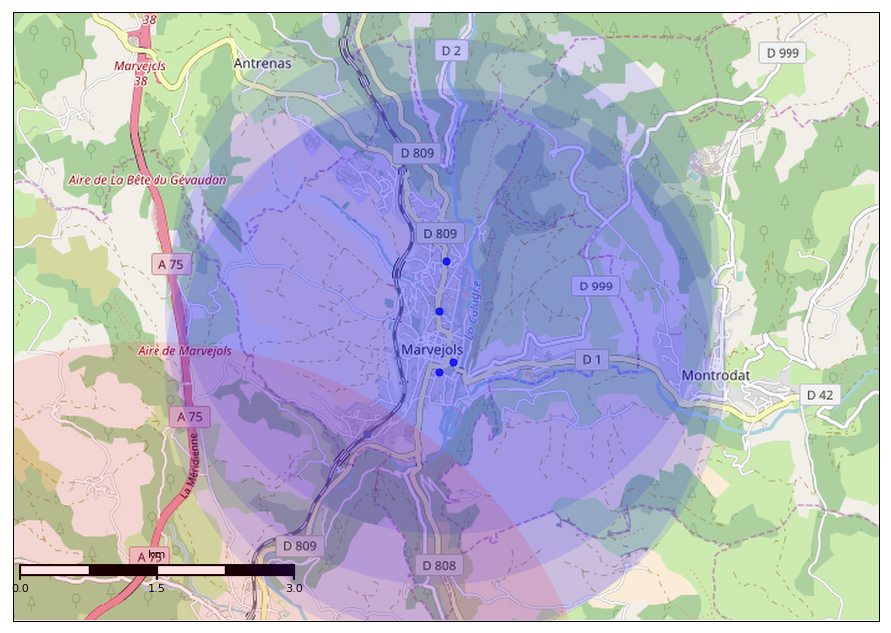
\includegraphics[width=1.1\textwidth]{graphs/case_study_marvejols_map.png}
\label{fig:case_study_map}
    \floatfoot{Background map from OpenStreetMap. Gas stations in the municipality of Marvejols (Loz\`ere)}
\end{figure}

The first part of the paper focuses on pairs of competing gas stations. More precisely, we consider all pairs of gas stations separated by a distance of less than 3 km and which are not operated by the same company. Figure~\ref{fig:case_study_map} provides the example of small municipality with four gas stations. Blue circles of 3 km radius are drawn around each gas station. Based on our definition of competition, all gas stations in the city compete with each other, which yields 6 pairs of competing gas stations. The part of the red circle in the lower left corner belongs to a 5km radius circle drawn around the gas station which is the closest to any of the gas stations in Marvejols. As a consequence, they are considered not to compete with gas stations outside of the municipality, even if we consider a distance of 5 km to define competition. The second part of the paper investigates price dispersion at the market level. Following a procedure previously used in the literature, we start by considering each gas station as the center of a market defined by a 3 km radius. In the case of Marvejols, this leads to define 4 markets which all contain the same outlets. We thus describe a simple procedure in section~\label{sec:market_dispersion} which allows to identify well defined markets such as the city of Marvejols.

\begin{figure}%[htb!]
    \caption{Retail diesel prices in Marvejols between November 2011 and November 2012}
	\centering
		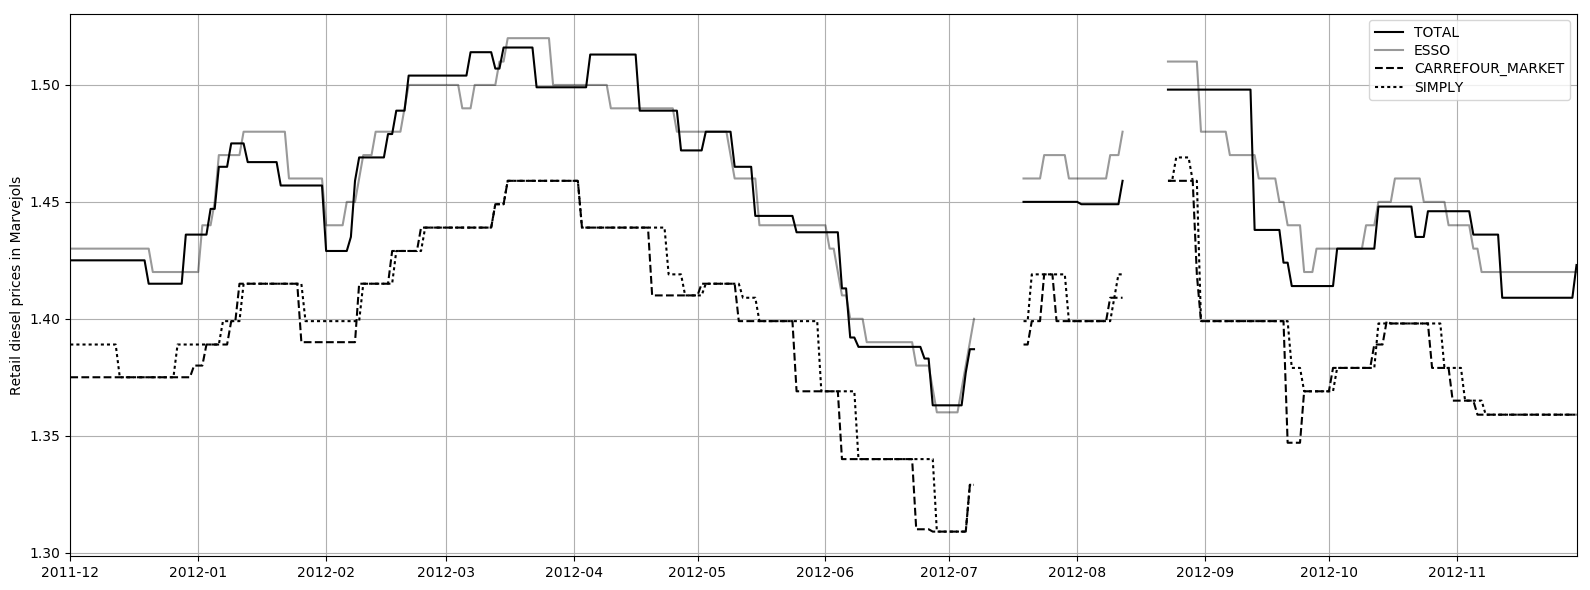
\includegraphics[width=\textwidth]{graphs/case_study_marvejols_prices.png}
\label{fig:case_study_prices}
\end{figure}

Figure~\ref{fig:case_study_prices} displays diesel prices in Marvejols between November 2011 and November 2012. Gas stations located the farthest north and south respectively belong to the Total and Esso chains. Their price levels can be seen to be relatively similar, and consistently higher than those of the Carrefour Market and Simply gas stations, which are both operated together with a supermarket. Prices at Carrefour Market and Simply are frequently perfectly aligned, while this is rarely the case for Total and Esso prices.

\section{Rank reversals, consumer information and leadership}

The goal of this section is to evaluate whether price dispersion a la \cite{VAR80} matches with price patterns observed in the French retail gasoline market.

\subsection{Rank reversals}

Randomization of prices in \cite{VAR80} means that a seller is cheaper or more expensive than a competitor with equal probabilities. The existence of such volatility in price rankings can be directly verified in the data. Furthermore, \cite{CHA11} suggest that we can test whether price dispersion and consumer search are connected based on the assumption that distance between sellers can be used as a proxy for search costs. The logic is that when a gas stations operates in the close vicinity of another, a higher share of consumers is likely to perfectly observe both prices than when sellers are separated by a higher distance. If the share of uninformed consumers is negligible, sellers can be expected to compete a la Bertrand, or Hotelling, and retail prices should essentially match wholesale price fluctuations. Conversely, if consumers are largely uninformed, dynamic dispersion can arise following the intuition exposed in \cite{VAR80}. \cite{CHA11} measure temporal price dispersion between two stations as the probability that the gas station which is in general cheaper, in terms of day count, turns out to be more expensive. Formally, denoting two gas stations $i$ and $j$, and $t \in T$ each day on which price records $p_{it}$ and $p_{jt}$ are available, the rank reversals statistic $r_{ij}$%
\footnote{All the statistics we use to account for price dispersion between pairs of gas stations are symmetric (in particular $r_{ij} = r_{ji}$).}%
writes:
\begin{align*}
r_{ij} = \min\left\{\frac{1}{T} \sum_{t=1}^{T} \mathbbm{1}_{p_{it} > p_{jt}}; \frac{1}{T} \sum_{t=1}^{T} \mathbbm{1}_{p_{jt} > p_{it}}\right\}
\end{align*}
Rank reversals can reach a maximum value of 50\% when gas station $i$ is strictly cheaper than its competitor $j$ during half of the period, and strictly more expensive during the other half. If one seller is always more expensive than the other, or both always set the same price, $r_{ij}$ takes value 0. In order to account for price alignment, we compute the percentage of days on which both sellers set the very same price:
\begin{align*}
sp_{ij} = \frac{1}{T} \sum_{t=1}^{T} \mathbbm{1}_{p_{it} = p_{jt}}
\end{align*}
Figure~\ref{fig:rr_pair_example} provides an example of two gas stations displaying large rank reversals. The Esso gas station is indeed successively more expensive and cheaper than its BP competitor between January and July 2014. The standard deviation of the daily price spread can be used as a proxy for dispersion that is robust to persistent price differences\footnote{Similarly as in \cite{CHA11}, we only perform this analysis with raw prices as rank reversals measured from price residuals tend to be highly sensitive to the process employed to obtain price residuals.}. Standard deviation is however more sensitive to outliers that can result from extraordinary promotions or erroneous price records. Formally, denoting $s_{ijt} = p_{it} - p_{jt}$ the price spread between gas station $i$ and $j$ on day $t$, and its average $\bar{s}_{ij} = \frac{1}{T} \sum_{t=1}^{T} s_{ijt}$, the standard deviation over the period is computed as follows:
\begin{align*}
\sigma_{ij} = \sqrt{\frac{1}{T} \sum_{t=1}^{T} [s_{ijt} - \bar{s}_{ij}]^2}
\end{align*}
We refer to $|\bar{s}_{ij}|$ as the long term average price difference or the mean price spread between two gas stations\footnote{This indicator is also symmetric: $|\bar{s}_{ij}| = |\bar{s}_{ji}|$.}.

\begin{figure}[htb!]
    \caption{Price series of two competing gas stations}
	\centering
		\includegraphics[width=\textwidth]{graphs/example_rr_93150003_93600010.png}
\label{fig:rr_pair_example}
\end{figure}

The formal test proposed by \cite{CHA11} consists in regressing measures of price dispersion on a dummy variable which identifies competitor pairs for which a low separating distance implies low search costs. Denoting $\text{Pair dispersion}_{ij}$ the price dispersion indicator between two gas stations $i$ and $j$, $\mathbbm{1}{\text{[Short distance]}_{ij}}$ an indicator for whether the stations are separated by a short distance, and $X_{ij}$ a set of control variables\footnote{Accordingly, $\beta_2$ is a vector of coefficients.}, the estimated equation:

\begin{equation}
\text{Pair dispersion}_{ij}= \beta_0 + \beta_1 \mathbbm{1}{\text{[Short distance]}_{ij}} + \beta_2 X_{ij} + \epsilon_{ij}
\end{equation}

Price dispersion, measured trough rank reversals or the standard deviation in prices, is expected to be lower when the separating distance is shorter, since information frictions are reduced. In the case where information is perfect, prices should be perfectly aligned as a result of Bertrand competition.

\subsection{Persistent price differences and spurious rank reversals}

Standard measures of market price dispersion are the range, namely the difference between the maximum and the minimum price, and the standard deviation of prices\footnote{Cf. \cite{BAY06} for a survey.}. As regards the French retail gasoline market, a naive use of these statistics is unlikely to be informative about search related price dispersion. Indeed, Total or BP gas stations are commonly expected to be much more expensive than a Leclerc or Carrefour gas station. The treatment of persistent price differences is a sensitive issue in the analysis of dispersion. It has been frequently addressed in the literature by working with price residuals, namely after controlling for seller (and occasionally time) fixed effects. However, beyond the practical errors inherent to the statistical treatment, this approach is only supported by theory to the extent that static price dispersion mirrors heterogeneity in offered utility\footnote{Cf. \cite{WIL11}.}. In our case, the large differences in prices and the relatively low predictive power of seller characteristics suggest that this represents a very strong assumption. Therefore, we consider an alternative hypothesis according to which a large persistent price difference between two retailers implies that they do not cater to the same customers. 

Two sources of large rank reversals unrelated to consumer information are identified in the data. One is the conversion by Total S.A. of nearly 300 Total gas stations to its discount brand, Total Access, accompanied by a sharp change in the pricing policy. Converted gas stations decrease prices by approximately 10 euro cents per liter, which has been found to trigger very moderate adjustments by competitors (\cite{CHA16}). A converted Total gas station is thus often consistently more expensive than a competitor at the beginning of the period and becomes cheaper once the conversion has occurred. Figure~\ref{fig:rr_total_access}, in appendix, provides such an example, for which a naive measure of rank reversals over the whole period is equal to 47\%. This issue is addressed by dropping all pairs of competitors which involve a Total gas stations converted to Total Access from our analysis\footnote{More generally, a similar phenomenon may arise whenever a shock affects a gas station differently from the way it affects its nearby competitors. The robustness of our results is tested i) by dropping gas stations which are found to implement a significant change in pricing policy over the period ii) by dropping pairs which exhibit high rank reversals but the price series of which scarcely cross each other. Details are available upon author request}. Another observed source of rank reversals is the occasional use by a few gas stations of dynamic price discrimination. The latter is detected by the regularity of successive inverse price changes at the gas station level. The most commonly observed pattern is a surge in prices during weekends. Such a pricing policy, whenever it is implemented unilaterally by a gas station in one market, can generate rank reversals which are unrelated to the use of mixed strategies. Figure~\ref{fig:rr_dynamic_price_discrimination}, in appendix, provides an illustration of the phenomenon. However, as very few observations are affected, dropping pairs of competitors which involve a gas station implementing dynamic price discrimination does not affect our results.

\subsection{Measured rank reversals}

For each pair of competing gas stations separated by a maximum distance of 3 km, we compute the percentages of rank reversals, same price, as well as the mean price spread and its standard deviation. This yields a database of 11,754 observations which are described in Table~\ref{tab:stats_pairs_3km}\footnote{Cf. Table~\ref{tab:stats_pairs_5km} in Appendix for replications with a distance of 5 km}. The average rank reversals is 7.1\% which is arguably small. Considering only pairs in which both retailers are either independent or operated by an oil company, the average rank reversals increases to 10.5\%. Within this sample, if we focus on pairs which exhibit a maximum mean price spread of 2 cents per liter, we are left with 646 pairs which exhibit an average 22.2\% rank reversals. These pairs can be noted to set the very same price on average 8.5\% of the time, while pairs of supermarket rivals (under the same spread restriction) respectively display a 32.2\% average probability to set the same price on a given day, and 14.6\% average rank reversals. Given the strong product homogeneity and the widely admitted competitive nature of the market, a reasonable baseline hypothesis for the strong price alignment displayed by many supermarket pairs is that involved gas stations compete \`{a} la Betrand. By contrast, pairs of high markup retailers, namely oil company and independent gas stations, often exhibit significant rank reversals, which make them good candidates for a theoretical representation in terms of MSE. By comparison, \cite{CHA11} report average rank reversals ranging from 11.9\% to 14.9\% with a maximum separating distance of 1 mile, and from 12.3\% to 15.9\% with 2 miles\footnote{They do not introduce restrictions on type or average price spread.}.

\begin{table}
\caption{Overview of pairs price dispersion (distance $\le$ 3 km)}
\label{tab:stats_pairs_3km}
\begin{threeparttable}
%\renewcommand{\arraystretch}{0.8} % too large by default...
%\small
\begin{tabular}{lrrrrr}
    \toprule
    \toprule
          & \multicolumn{1}{c}{Nb} & \multicolumn{1}{c}{Rank} & \multicolumn{1}{c}{Same} & \multicolumn{2}{c}{Price spread} \\
          & \multicolumn{1}{c}{pairs} & \multicolumn{1}{c}{reversals} & \multicolumn{1}{c}{price} & \multicolumn{1}{c}{Mean} & \multicolumn{1}{c}{Std.} \\
    \midrule
    No price spread restriction &       &       &       &       &  \\
    All types & 11 754 & 7.1 (10.8) & 7.8 (17.0) & 5.3 (4.3) & 1.6 (0.6) \\
    - Oil \& Ind & 1 679 & 10.5 (12.0) & 3.9 \phantom{0}(9.0) & 3.2 (2.6) & 1.9 (0.6) \\
    - Supermarkets \& Discounters & 3 706 & 15.4 (11.3) & 21.7 (23.6) & 1.0 (1.0) & 1.3 (0.5) \\
    \hspace*{4mm} - Supermarkets & 2 232 & 12.9 (10.3) & 27.3 (27.6) & 1.0 (1.1) & 1.3 (0.5) \\
    \hspace*{4mm} - Discounters & 157   & 28.2 \phantom{0}(9.5) & 13.6 \phantom{0}(6.5) & 0.4 (0.4) & 1.1 (0.3) \\
    \hspace*{4mm} - Supermarkets vs. discounters & 1 317 & 18.1 (11.4) & 13.1 (11.7) & 1.0 (0.9) & 1.3 (0.5) \\
    \midrule
    Price spread <= 2 cent per liter &       &       &       &       &  \\
    All types & 4 171 & 18.1 (11.3) & 21.3 (23.0) & 0.7 (0.6) & 1.3 (0.5) \\
    - Oil \& Ind & 646   & 22.2 (10.7) & 8.5 (13.1) & 1.1 (0.5) & 1.7 (0.4) \\
    - Supermarkets \& Discounters & 3 176 & 17.1 (11.1) & 24.9 (24.0) & 0.6 (0.5) & 1.2 (0.4) \\
    \hspace*{4mm} - Supermarkets & 1 867 & 14.6 (10.3) & 32.2 (27.6) & 0.6 (0.5) & 1.2 (0.5) \\
    \hspace*{4mm} - Discounters & 156   & 28.3 \phantom{0}(9.4) & 13.7 \phantom{0}(6.5) & 0.4 (0.4) & 1.1 (0.3) \\
    \hspace*{4mm} - Supermarkets vs. discounters & 1 153 & 19.8 (11.0) & 14.6 (11.7) & 0.7 (0.5) & 1.2 (0.4) \\
    \midrule
    Price spread <= 1 cent per liter &       &       &       &       &  \\
    All types & 2 928 & 20.3 (11.8) & 27.4 (24.6) & 0.4 (0.3) & 1.1 (0.4) \\
    - Oil \& Ind & 297   & 29.0 (10.5) & 12.1 (17.0) & 0.5 (0.3) & 1.6 (0.4) \\
    - Supermarkets \& Discounters & 2 423 & 19.0 (11.5) & 30.2 (24.9) & 0.4 (0.3) & 1.1 (0.4) \\
    \hspace*{4mm} - Supermarkets & 1 404 & 15.9 (10.8) & 40.0 (17.3) & 0.3 (0.3) & 1.1 (0.4) \\
    \hspace*{4mm} - Discounters & 140   & 30.0 \phantom{0}(8.2) & 14.4 \phantom{0}(6.4) & 0.3 (0.2) & 1.0 (0.3) \\
    \hspace*{4mm} - Supermarkets vs. discounters & 879   & 22.2 (10.9) & 17.1 (11.9) & 0.5 (0.3) & 1.1 (0.3) \\
    \bottomrule
    \bottomrule
\end{tabular}
\begin{tablenotes}
			\small
      \item Except for the first column, all figures are averages of statistics computed at the pair level (standard errors in parentheses). "Mean Price spread" refers to $|\bar{s}_{ij}|$ and accounts for the existence of persistent price differences (0 if both gas stations are equally expensive over the long term), while the standard deviation, "Std. Price spread", measures dispersion around the long term price difference (0 if both gas stations always set the same price). "Rank reversals" and "Same price" are percentages.
\end{tablenotes}
\end{threeparttable}
\end{table}

Figure~\ref{fig:pct_reversed_pairs}, in appendix, displays the percentage of pairs of gas stations whose price rank is reversed on each day of the period studied. Among pairs of gas stations built with a maximum distance of 3 km, the percentage of reversed pairs fluctuates between 5.4\% and 15.3\%  (mean 8.1\%). The ``No differentiation'' series results from a focus on pairs which exhibit an average price difference below 2c/l. Among these pairs, the minimum percentage of reversed pairs fluctuates between 13.8\% and 29.3\% (mean 19.5\%). From a consumer viewpoint, this translates in one chance in five to pay the highest price upon patronizing among two competitors of similar price level the one which is cheaper most of the time.

\subsection{Test of the relation with consumer information}

A clear ranking of empirical distribution functions of rank reversals can be observed among pairs of gas stations depending on distances in Figure~\ref{tab:ecdf_rr_distance}. This is consistent with the idea that nearby gas stations compete in a virtually complete information setting, in which there is no reason to expect rank reversals. Conversely, distance can create an information issue for other pairs, preventing the existence of an equilibrium in pure strategy.

\begin{figure}[H]
\centering
\caption{Empirical distribution functions of rank reversals}
\label{tab:ecdf_rr_distance}
\begin{subfigure}{.49\textwidth}
\centering
\includegraphics[width=\textwidth]{graphs/ecdf_rank_reversals_le_2c.png}
\caption[short]{Pair average price spread $\le$ 2 cent/litre}
\end{subfigure}
\begin{subfigure}{.49\textwidth}
\centering
\includegraphics[width=\textwidth]{graphs/ecdf_rank_reversals_le_1c.png}
\caption[short]{Pair average price spread $\le$ 1 cent/litre}
\end{subfigure}
\end{figure}

Table~\ref{tab:regs_pairs} reports the estimations of $\beta_1$ obtained with all competitor pairs as well as subsamples based on gas station types, using both rank reversals and standard deviation in spread as proxies for pair price dispersion. Overall, pairs of gas stations which are separated by a distance of 1 km or less exhibit rank reversals which are 2.3 points smaller than pairs which are separated by a distance comprised between 1 and 3 km. This result is close to the 2.7 point difference found by \cite{CHA11}. The average effect is stronger for pairs of oil and independent gas stations, and smaller for supermarkets. For the latter, no significant impact is found when standard deviation in spread is used to account for price dispersion. Considering the relative strong price alignment displayed by supermarket pairs, this leads to put into perspective the impact of consumer search cost on their markets\footnote{Theoretically, rank reversals with strong price alignment can be obtained in an extension of \cite{VAR80} that requires sellers to choose prices from a grid. Occasional rank reversals could also simply result from temporary frictions linked to wholesale cost variations, or short periods of price wars.}. 

\begin{table}%[hbtp]
\caption{Regressions of pair price dispersion (average price spread $\le$ 1 euro cent per liter)}
\label{tab:regs_pairs}
%\renewcommand{\arraystretch}{0.8} % too large by default...
\begin{threeparttable}
    \begin{tabular}{rrrrrrr}
    \toprule
    \toprule
          & \multicolumn{1}{l}{Dependent} &       & \multicolumn{4}{c}{Quantile regressions} \\
          & \multicolumn{1}{l}{Variable} & OLS   & 25\%  & 50\%  & 75\%  & 90\% \\
    \midrule
    \multicolumn{1}{l}{All pairs} & \multicolumn{1}{l}{$r_{ij}$} & -2.28*** & -1.70*** & -3.60*** & -2.70*** & -2.10*** \\
    \multicolumn{1}{l}{(N =  2 928)} &       & (0.51) & (0.66) & (0.86) & (0.80) & (0.81) \\
          & \multicolumn{1}{l}{$\sigma_{ij}$} & -0.04** & -0.05*** & -0.03 & -0.02 & -0.01 \\
          &       & (0.02) & (0.02) & (0.02) & (0.03) & (0.04) \\
    \midrule
    \multicolumn{1}{l}{Oil \& Ind} & \multicolumn{1}{l}{$r_{ij}$} & -3.29** & -3.80** & -3.00* & -1.90 & -0.50 \\
    \multicolumn{1}{l}{ (N = 297)} &       & (1.34) & (1.82) & (1.74) & (1.84) & (1.84) \\
          & \multicolumn{1}{l}{$\sigma_{ij}$} & -0.22*** & -0.25*** & -0.21*** & -0.17* & -0.10 \\
          &       & (0.05) & (0.06) & (0.06) & (0.09) & (0.12) \\
    \midrule
    \multicolumn{1}{l}{Supermarkets} & \multicolumn{1}{l}{$r_{ij}$} & -2.12*** & -1.40** & -2.50*** & -2.30 & -1.90 \\
    \multicolumn{1}{l}{ (N = 1 404)} &       & (0.68) & (0.60) & (0.91) & (1.41) & (1.60) \\
          & \multicolumn{1}{l}{$\sigma_{ij}$} & -0.01 & -0.02 & -0.01 & 0.04  & -0.02 \\
          &       & (0.02) & (0.03) & (0.03) & (0.04) & (0.05) \\
    \midrule
    \multicolumn{1}{l}{Discounters} & \multicolumn{1}{l}{$r_{ij}$} & -2.29 & -2.80 & -1.10 & -3.10 & -2.80 \\
    \multicolumn{1}{l}{ (N = 140)} &       & (1.69) & (2.96) & (2.44) & (2.15) & (2.23) \\
          & \multicolumn{1}{l}{$\sigma_{ij}$} & -0.28*** & -0.19*** & -0.24*** & -0.38*** & -0.52*** \\
          &       & (0.06) & (0.07) & (0.08) & (0.08) & (0.10) \\
    \midrule
    \multicolumn{1}{l}{Supermarkets vs. Discounters} & \multicolumn{1}{l}{$r_{ij}$} & -2.70*** & -3.40** & -2.80** & -2.60** & -4.30*** \\
    \multicolumn{1}{l}{(N = 879)} &       & (0.91) & (1.49) & (1.34) & (1.32) & (1.31) \\
          & \multicolumn{1}{l}{$\sigma_{ij}$} & -0.02 & -0.05* & -0.03 & 0.00  & 0.02 \\
          &       & (0.03) & (0.03) & (0.03) & (0.04) & (0.07) \\
    \bottomrule
    \bottomrule
\end{tabular}
\begin{tablenotes}
      \small
      \item Standard errors in parentheses. Significance thresholds: * p<.1, ** p<.05, *** p<.01.
\end{tablenotes}
\end{threeparttable}
\end{table}

Overall, empirical findings provide support for the existence of price dispersion related to consumer search, but we also observe that most low markup gas stations tend to largely align prices with those of nearby competitors. While this could simply reflect almost perfect consumer information, one must take into account the fact that supermarkets may use gasoline to attract consumers in stores, thus setting prices in a way that does not purely reflect fundamental local market characteristics. We discuss this question through an analysis of price alignment and chain affiliation.

\subsection{Leadership: the importance of chain affiliation}

Several papers in the literature have emphasized how chain strategies can shape market prices and dynamics. \cite{HOS08} remark that gas stations of a specific chain nearly always match the lowest price in their local market. \cite{LEW12}, working on markets which exhibit Edgeworth cycles, show that gas stations of two chains exhibit a much higher probability of jumping on the first day of the restoration than most of their competitors. They also show that cycles tend to be absent from almost every city in which these two chains have little or no market presence.

In order to capture the potential existence of leadership in price changes, we count, within each pair, the number of times each seller matches the price of its competitor. Formally, the number of times seller $i$ matches the price of seller $j$ writes:

\begin{align*}
\sum_{t=2}^{T}\mathbbm{1}_{p_{it} = p_{jt} \text{ with } p_{it-1} \neq p_{jt-1} \text{ and } p_{jt} = p_{jt-1}}
\end{align*}
We then test the hypothesis that each gas station is equally likely to match its competitor's price through a binomial test of equality of the two statistics\footnote{Cf. \cite{SEA13} for a similar approach with British supermarket prices.}. Whenever the equality hypothesis is rejected, the gas station which displays the highest figure is considered as a leader, and the other as a follower\footnote{Sellers are often observed to simultaneously adopt the same price on a given day. Such observations are not taken into account in the test.}. Regarding pairs for which the equality hypothesis is not rejected, we want to consider only pairs which actually often set the same price. We thus drop pairs which do not meet a threshold regarding the percentage of days on which both gas stations set the same price. Figure~\ref{fig:leader_pair_example} displays the price series of a pair in which leadership is detected. The Intermarche gas station can be seen to frequently match the price of a Leclerc competitor. Each vertical dashed line corresponds to one such adjustment.

\begin{figure}[htb!]
    \caption{Example of two gas stations identified as leader and follower}
	\centering
		\includegraphics[width=\textwidth]{graphs/example_leadership_1700004_1120005.png}
\label{fig:leader_pair_example}
\flushleft
\small
The Intermarche gas station can be seen to frequently match the price of its Leclerc competitor. Each vertical dashed line corresponds to one such adjustment.
\end{figure}

Results are aggregated for each gas station in order to distinguish those which have at least one competitor with similar prices, and among those to evaluate which ones can be identified as leaders or followers in their market. A gas station is labeled as a relative leader, respectively follower, when it is found to lead, respectively follow, in at least one pair. Furthermore, all gas stations belonging to pairs in which no leader can be identified are labeled as uncertain. Importantly, these three labels are not mutually exclusive: a gas station can identified as a leader in one pair, a follower in another, and neither as a leader nor a follower in a third. Finally, an absolute leader is defined as a seller which belongs to the set of relative leaders but not to the sets of relative followers and uncertain. Similarly, an absolute follower is defined as a seller which belongs to the set of relative followers but not to the sets of relative leaders and uncertain. Gas stations which exclusively belong to pairs for which no leader is identified are labeled as absolutely uncertain. The daily frequency of the data imposes a limitation on leadership detection. Many pairs which are labeled uncertain by the present analysis may be found to involve leadership if the exact time of price changes was taken into account. Unfortunately, such inaccuracies tend to propagate across observations. When a gas station $A$ matches the prices of a competitor $B$ so closely that no leader is identified, if a seller $C$ loosely follows $B$, both $A$ and $B$ are labeled as relative leaders in their comparison with $C$. Results analyzed at the chain level however suggest that the present analysis, despite its current limitations, conveys meaningful information.

\begin{table}%[hbtp]
\caption{Overview of leadership test results by chain}
\label{tab:stats_leadership}
%\renewcommand{\arraystretch}{0.8} % too large by default...
%\small
\begin{threeparttable}
    \begin{tabular}{llr|r|rr|rr|rr}
\toprule
\toprule
    Type   &  Chain     & \multicolumn{1}{l|}{Nb} & \multicolumn{1}{l|}{Similar} & \multicolumn{2}{c|}{Leader} & \multicolumn{2}{c|}{Follower} & \multicolumn{2}{c}{Uncertain} \\
           &            & \multicolumn{1}{l|}{stations} & \multicolumn{1}{l|}{prices} & \multicolumn{1}{l}{Rel.} & \multicolumn{1}{l|}{St.} & \multicolumn{1}{l}{Rel.} & \multicolumn{1}{l|}{St.} & \multicolumn{1}{l}{Rel.} & \multicolumn{1}{l}{St.} \\
    \midrule
    \multicolumn{2}{l}{\textbf{Oil/Independent}}  &       &       &       &       &       &       &       &  \\
    Oil   & Total & 1 365 & 7     & 1     & 1     & 1     & 1     & 4     & 4 \\
    Oil   & Elan (Total) & 279   & 5     & 1     & 1     & 0     & 0     & 4     & 4 \\
    Oil   & Agip  & 132   & 14    & 1     & 1     & 6     & 5     & 9     & 8 \\
    Oil  & BP    & 290   & 7     & 1     & 1     & 1     & 1     & 6     & 5 \\
    Oil  & Esso  & 156   & 15    & 3     & 2     & 2     & 2     & 12    & 10 \\
    Independent & Avia  & 403   & 18    & 2     & 2     & 5     & 3     & 13    & 11 \\
    Independent & Dyneff & 64    & 14    & 5     & 0     & 5     & 2     & 11    & 6 \\
    Independent & Other & 390   & 27    & 6     & 3     & 5     & 3     & 22    & 17 \\
    \midrule
    \multicolumn{2}{l}{\textbf{Oil discount}}       &       &       &       &       &       &       &       &  \\
    Oil discount & Total access & 319   & 34    & 19    & 16    & 8     & 6     & 12    & 8 \\
    Oil discount & Esso express & 326   & 63    & 6     & 2     & 45    & 29    & 31    & 15 \\
    \midrule
    \multicolumn{2}{l}{\textbf{Supermarkets}} &       &       &       &       &       &       &       &  \\
    Large & Carrefour & 198   & 94    & 37    & 1     & 73    & 19    & 62    & 12 \\
    Large & Auchan & 119   & 83    & 63    & 24    & 29    & 6     & 49    & 8 \\
    Large & Cora  & 115   & 43    & 24    & 9     & 14    & 3     & 30    & 10 \\
    Large & Geant Casino & 97    & 96    & 34    & 6     & 81    & 19    & 63    & 5 \\
    Large/medium & Intermarche & 1 392 & 43    & 19    & 12    & 16    & 7     & 22    & 11 \\
    Large/medium & Systeme U & 773   & 47    & 19    & 9     & 19    & 9     & 28    & 14 \\
    Large/medium & Leclerc & 591   & 75    & 58    & 35    & 9     & 3     & 35    & 12 \\
    Medium & Carrefour market & 704   & 62    & 8     & 2     & 47    & 31    & 26    & 11 \\
    Small & Carrefor contact & 236   & 11    & 2     & 1     & 2     & 1     & 9     & 8 \\
    Small & Simply (Auchan) & 226   & 24    & 10    & 7     & 6     & 4     & 13    & 8 \\
    Small & Casino & 206   & 24    & 4     & 2     & 15    & 12    & 9     & 7 \\
    Small & Intermarche contact & 116   & 24    & 7     & 5     & 5     & 4     & 15    & 12 \\
    Other & Other & 224   & 29    & 6     & 3     & 9     & 6     & 21    & 14 \\
    \bottomrule
    \bottomrule
\end{tabular}
%\begin{tablenotes}
%\end{tablenotes}
\end{threeparttable}
\end{table}

Table~\ref{tab:stats_leadership} reports results aggregated at the chain level. The column ``Similar prices'' provides the percentage of gas stations within each chain which have at least one competitor exhibiting similar prices, namely with which they set the same price more than 30\% of the time. The ``Relative Leader'' column provides the percentage of gas stations within each chain which are identified as relative leaders in at least one pair. The ``Strict Leader'' column provides the percentage of gas stations within each chain which are identified as strict leaders in their market. Oil company and independent gas stations are confirmed to be relatively less likely than others to align prices with competitors. Conversely, many gas stations operated by large supermarkets have competitors which frequently adopt the same prices. For instance, respectively 73\% and 58\% of gas stations operated by Carrefour and Leclerc\footnote{Carrefour and Leclerc are the two leading food retailers in France}, are found to compete with at least one seller with which they share the same price 30\% of the time or or more. The same is true for oil discounters, while smaller supermarket chains exhibit figures which are significantly lower, yet remaining higher than those of oil company gas stations.
Leclerc, which is widely acknowledged to be the most aggressive large retailer regarding prices, is by far the chain under which the share of absolute leaders is the highest (35\%). The only other chain to exhibit a share of absolute leaders above 10\% is Auchan (23\%). Carrefour gas stations, on the other hand, appear much more likely to act as followers (26\% are labelled absolute followers for large supermarkets, and respectively 29\% for medium size supermarkets), as are Geant Casino stores (33\% absolute followers). Results for Systeme U and Intermarche are more balanced, which is likely reflects the strong heterogeneity in store formats. These two chains also differ from Auchan, Carrefour and Geant by being franchises, as opposed to integrated groups. Finally, results suggest that Total Access are much more likely to lead, conversely to Esso Express gas stations which are more frequently found to follow. A possible explanation may lie in the ownership structure of Esso Express gas stations, as slower price adjustments could be linked to vertical contracting, or to the creation of the chain Total Access over the period. Prices at converted gas stations were indeed more likely to be under scrutiny, thus creating an incentive to price relatively aggressively\footnote{Under the current test, a gas station which cuts prices quickly when the cost of wholesale diesel drops, and does not lag behind when it goes up, will typically be identified as a leader (even though it may only initiate price cuts).}.

To conclude, the analysis of price leadership suggests that gas station chain affiliation often plays an important role in shaping market prices. Concerned gas stations are mostly operated by supermarkets, which is consistent with gasoline prices being used to attract consumers in stores. This leads to be cautious regarding the possibility to conclude that strong price alignment reflects virtually perfect consumer information. Nevetheless, such a reserve does not applied to discount gas stations. Overall, low markup gas stations thus appear to generally compete for a well informed highly price sensitive demand.

\section{Price dispersion, cost and number of firms}
\label{sec:market_dispersion}

The following section investigates how variations in cost and competition intensities relate to market price dispersion. The first approach consists in working with measures of price dispersion for each local market and day. As it requires relatively strong assumptions regarding the definition of markets and the reliability of dispersion measures, the richness of the data is used to measure price dispersion directly at the gas station level, from each price distribution. This allows to gather additional evidence on the link between competition and dispersion.

The first approach closely follows \cite{CHA11}. Each gas station is successively considered as the center of a market delimited by a circle of a given radius. Price dispersion is then measured on each day as the empirical range and standard deviation of local prices. This allows to investigate how price dispersion varies with cost variations over time on the one hand, and with the intensity of competition across markets on the other hand. As noted by \cite{CHA11}, results regarding competition must yet be analyzed with caution. The number of gas stations within an area indeed reflects demand and thus may not provide an accurate measure of the competitiveness of the market. Also, considering each gas station as the center of a market leads to attribute a lot of weight to markets which exhibit high seller densities. To tackle this issue, a simple algorithm is used to obtain non overlapping markets. We impose that i) each gas station in the market competes directly, or indirectly via another seller, with all other retailers in the market, using a 3 km threshold to define competition ii) no gas station which is not part of the market should be within 5 km of a gas station in the market. The first criterion thus ensures that all retailers in the market are close enough to each other, while the second requires the market to be relatively isolated from the closest sellers which are not part of it. This algorithm leads to identify 508 local markets, with no gas station being part of two markets.

Finally, we deal with persistent price differences by working with residual prices, namely prices net of station-specific fixed effects. Furthermore, besides following an approach which supposes that all gas stations compete in the same market, we consider a scenario involving market segmentation. Oil and independent gas stations are then assumed to compete in high price markets, while supermarket and discount gas stations form low price markets.

Table~\ref{tab:stats_des_markets} reports descriptive statistics of price dispersion at the market level. All measures of price dispersion can be seen to drop significantly when residual prices are used and under the market segmentation scenario. For instance, under the simple 3 km radius market definition, gains from search, are estimated to be 1.25 euro cents per liter with residual prices while they were 3.93 euro cents per liter with raw prices. Under segmentation, dispersion is higher within high price gas station markets (2.90 vs. 0.97 euro cents per liter gains from search with raw prices). The variations observed between dispersion measures computed with raw and residual prices confirm than high price gas stations tend to be more differentiated than low price gas stations.

\begin{table}%[H]
\caption{Market-level summary statistics}
\label{tab:stats_des_markets}
%\renewcommand{\arraystretch}{0.8} % too large by default...
%\small
\begin{threeparttable}
\begin{tabular}{lrrrr}
    \toprule
    \toprule
          & \multicolumn{1}{c}{All} & \multicolumn{1}{c}{Low} & \multicolumn{1}{c}{High} & \multicolumn{1}{c}{No overlap} \\
    \midrule
    Nb observations & \multicolumn{1}{c}{3 838 661} & \multicolumn{1}{c}{1 345 825} & \multicolumn{1}{c}{ 509 245} & \multicolumn{1}{c}{ 539 548} \\
    Nb markets & \multicolumn{1}{c}{ 3 605} & \multicolumn{1}{c}{ 1 262} & \multicolumn{1}{c}{  492} & \multicolumn{1}{c}{  508} \\
    \midrule
    Nb sellers & 5.09 (2.61) & 3.96 (1.34) & 4.75 (2.43) & 4.17 (1.82) \\
    Nb sellers observed & 4.88 (2.51) & 3.85 (1.35) & 4.47 (2.31) & 3.99 (1.80) \\
    \midrule
    \multicolumn{2}{l}{Raw prices (euro cents per liter)} &       &       &  \\
    Range & 9.17 (4.44) & 2.14 (1.86) & 5.47 (3.31) & 8.54 (4.58) \\
    Standard deviation & 3.71 (1.76) & 0.87 (0.75) & 2.11 (1.20) & 3.65 (1.96) \\
    Gain from search & 3.68 (2.08) & 0.94 (0.85) & 2.71 (1.67) & 3.38 (2.02) \\
    \midrule
    \multicolumn{2}{l}{Residual prices (euro cents per litre)} &       &       &  \\
    Range & 2.26 (1.62) & 1.60 (1.34) & 2.53 (1.68) & 1.96 (1.49) \\
    Standard deviation & 0.84 (0.57) & 0.64 (0.53) & 0.96 (0.61) & 0.78 (0.58) \\
    Gain from search & 1.13 (0.87) & 0.79 (0.70) & 1.25 (0.90) & 0.98 (0.81) \\
\bottomrule
\bottomrule
\end{tabular}
\begin{tablenotes}
      \small
      \item Standard errors in parentheses.
\end{tablenotes}
\end{threeparttable}
\end{table}

With $\text{Market Dispersion}_{jt}$ a measure of price dispersion on market $j$ at date $t$, $Trend_t$ a trend variable, $MC_t$ a measure of the marginal cost (wholesale diesel in euro per liter) on date $t$, $N_j$ the number of gas stations on market $j$, we estimate the parameters of the following equation for each market definition:

\begin{equation}
\text{Market Dispersion}_{jt}= \beta_0 + \beta_1 Trend_t + \beta_2 MC_t + \beta_2 N_j + \epsilon_{jt}
\end{equation}

Considering that the government intervention between August 2012 and January 2013 may have had a relatively strong temporary impact on dispersion, in a period of high oil prices, estimation outputs are provided in Table~\ref{tab:regs_market_dispersion_after} for the period starting February 1, 2013 (628 days). They are consistent with results obtained by \cite{CHA11}: dispersion is found to increase with the number of firms and decrease with cost. Cost appears to have a stronger impact on dispersion displayed by high markup gas stations than low markup gas stations. When the whole period is considered (cf. Table~\ref{tab:regs_market_dispersion_after} in appendix), cost is estimated to have a significant impact only for high markup gas stations. This result is consistent with fierce price competition among low markup gas stations, and more relaxed competition, in a context of imperfect information, for oil company and independent gas stations.

\begin{table}%[H]
\caption{Regressions of market dispersion}
\label{tab:regs_market_dispersion_after}
%\renewcommand{\arraystretch}{0.8} % too large by default...
%\small
\begin{threeparttable}
    \begin{tabular}{lrrrrrrrr}
    \toprule
    \toprule
          & \multicolumn{2}{c}{All} & \multicolumn{2}{c}{Low} & \multicolumn{2}{c}{High} & \multicolumn{2}{c}{No overlap} \\
          & \multicolumn{1}{c}{Range} & \multicolumn{1}{c}{Std} & \multicolumn{1}{c}{Range} & \multicolumn{1}{c}{Std} & \multicolumn{1}{c}{Range} & \multicolumn{1}{c}{Std} & \multicolumn{1}{c}{Range} & \multicolumn{1}{c}{Std} \\
    \midrule
    Constant & 6.21*** & 2.49*** & 3.55*** & 1.62*** & 6.62*** & 2.77*** & 5.98*** & 2.54*** \\
          & (1.51) & (0.58) & (1.38) & (0.56) & (1.20) & (0.49) & (1.57) & (0.64) \\
    Trend & -0.00** & -0.00** & -0.00 & -0.00 & -0.00*** & -0.00*** & -0.00** & -0.00** \\
          & (0.00) & (0.00) & (0.00) & (0.00) & (0.00) & (0.00) & (0.00) & (0.00) \\
    Cost  & -7.94*** & -2.90*** & -4.38* & -1.76* & -8.50*** & -3.28*** & -7.55*** & -2.95*** \\
          & (2.19) & (0.84) & (2.01) & (0.82) & (1.76) & (0.71) & (2.26) & (0.91) \\
    Nb firms & 0.24*** & 0.04*** & 0.27*** & 0.06*** & 0.27*** & 0.05*** & 0.22*** & 0.04*** \\
          & (0.01) & (0.00) & (0.01) & (0.00) & (0.02) & (0.01) & (0.02) & (0.01) \\
    \midrule
    R2    & 0.19  & 0.07  & 0.12  & 0.06  & 0.21  & 0.09  & 0.10  & 0.04 \\
    N     & 632 765 & 632 765 & 222 438 & 222 438 & 83 076 & 83 076 & 88 565 & 88 565 \\
\bottomrule
\bottomrule
\end{tabular}
\begin{tablenotes}
      \small
      \item Standard errors in parentheses, clustered by market and date.
      \item Significance thresholds: * p<.1, ** p<.05, *** p<.01.
      \item Region fixed effects are included in all specifications.
\end{tablenotes}
\end{threeparttable}
\end{table}

This approach however has significant shortcomings. First, it leaves out gas stations which have no or few competitors around, and either tends to give much weight to large markets, or to restrict the analysis to a limited number of markets, the definition of which remains uncertain. The empirical range is a relatively volatile statistic, and the empirical standard deviation is generally a biased estimator (absent knowledge of the distribution), which typically leads to underestimate actual standard deviation when samples are small. As a consequence, we develop another approach which consists in measuring dispersion directly from the residual price distribution of each seller. An important merit lies in the fact that potential outliers can be dropped easily (either by trimming the price distribution, or by dropping seller dispersion statistics ex-post). Measures of price dispersion thereby obtained are reported in Table~\ref{tab:station_price_support_stats_des}.

\begin{table}[H]
\caption{Gas station residual price distributions}
\label{tab:station_price_support_stats_des}
%\renewcommand{\arraystretch}{0.8} % too large by default...
%\small
\begin{threeparttable}
\begin{tabular}{lrrr}
    \toprule
    \toprule
          & \multicolumn{1}{c}{Oil/Ind} & \multicolumn{1}{c}{Discount} & \multicolumn{1}{c}{Supermarkets} \\
    \midrule
    Nb stations & \multicolumn{1}{c}{1 457} & \multicolumn{1}{c}{476} & \multicolumn{1}{c}{3 995} \\
    Std   & 1.11 (0.39) & 1.00 (0.29) & 1.06 (0.28) \\
    Kurtosis & 1.15 (3.79) & 1.43 (3.81) & 2.77 (3.91) \\
    Skewness & 0.07 (0.69) & 0.20 (0.74) & -0.55 (0.87) \\
    Range & 6.65 (2.04) & 6.24 (1.77) & 7.53 (2.03) \\
    Trimmed range 5\% & 4.25 (1.43) & 3.87 (1.13) & 4.14 (1.16) \\
    Trimmed range 10\% & 3.52 (1.23) & 3.18 (0.96) & 3.29 (0.93) \\
    \bottomrule
    \bottomrule
\end{tabular}
\begin{tablenotes}
      \small
      \item Standard errors in parentheses.
\end{tablenotes}
\end{threeparttable}
\end{table}

Price distributions of supermarket gas station exhibit smaller standard deviations but fatter tails than these of oil and independent gas stations. They are generally left-skewed, which reflects the (scarce) use of promotions, often implemented at the chain level. Conversely, no systematic skew is observed for oil and independent gas stations. In order to investigate the relation between price dispersion and seller density, the empirical standard deviation and the range are regressed on the number of competitors within 3 km.

\begin{table}[H]
\caption{Regressions of price dispersion measured at the gas station level}
\label{tab:station_price_support_regs}
%\renewcommand{\arraystretch}{0.8} % too large by default...
%\small
\begin{threeparttable}
\begin{tabular}{lrrrrrr}
    \toprule
    \toprule
          & \multicolumn{2}{c}{Oil} & \multicolumn{2}{c}{Discount} & \multicolumn{2}{c}{Supermarkets} \\
          & \multicolumn{1}{c}{Tr. range} & \multicolumn{1}{c}{Std} & \multicolumn{1}{c}{Tr. range} & \multicolumn{1}{c}{Std} & \multicolumn{1}{c}{Tr. range} & \multicolumn{1}{c}{Std} \\
    \midrule
    Constant & 3.83*** & 1.00*** & 3.51*** & 0.92*** & 3.94*** & 1.03*** \\
          & (0.03) & (0.01) & (0.11) & (0.03) & (0.02) & (0.01) \\
    Nb firms & 0.05*** & 0.02*** & 0.04  & 0.01  & 0.01  & 0.00 \\
          & (0.01) & (0.00) & (0.04) & (0.01) & (0.01) & (0.00) \\
    \midrule
    R2    & 0.11  & 0.13  & 0.11  & 0.12  & 0.04  & 0.08 \\
    N     & 1 735 & 1 735 &  476  &  476  & 3 995 & 3 995 \\
    \bottomrule
    \bottomrule
\end{tabular}
\begin{tablenotes}
      \small
      \item Standard errors in parentheses. Significance thresholds: * p<.1, ** p<.05, *** p<.01.
      \item Region fixed effects are included in all specifications.
\end{tablenotes}
\end{threeparttable}
\end{table}

Regression results in Table~\ref{tab:station_price_support_regs} lead to question the results obtained with the previous specification. Seller density is no more found to have an impact on price dispersion for supermarkets and discounters. A significant positive relationship is yet still found for oil and independent gas stations. Estimates do not significantly differ whether seller density is accounted for by the number of competitors of the same type or by all competitors. Such results are relatively consistent with previous findings on the link between consumer information and dispersion. Indeed, supermarkets were found to often be engaged in tough price competition, leaving little room for the extraction of an informational rent. Conversely, consumer search seemed to play a bigger role in the case of oil and independent gas stations, so that a positive relationship between dispersion and competition intensity could be expected based on a model a la \cite{VAR80}.

\section{Conclusion}

This paper analyzes price dispersion in the French retail gasoline market, taking into account the presence of large persistent price differences between gas stations, with supermarket and discount gas stations setting prices generally 8 to 10 euro cents per liter cheaper than oil company and independent gas stations. Overall, rank reversals are  found to be less frequent for pairs of retailers separated by a short distance, namely competitors whose prices are easy to compare for consumers. This result supports the hypothesis of a connection between consumer information and price dispersion. Pairs of competitors which operate at low markups, namely supermarkets and discounters, exhibit less rank reversals than those which sell at higher markups. Pairs of competitors operating at low markups are often observed to adopt the very same prices with a high probability. The study of price dynamics allows to unveil large scale price leadership, which is strongly correlated with chain affiliation. Conversely, high markup gas stations tend to exhibit significant dynamic price dispersion. This leads us to conclude that the latter generally address the needs of customers characterized by relatively strong loyalty or high search costs, while supermarkets compete for a well informed highly price sensitive demand.

At the market level, due to large persistent differences in gas station markups, working with raw prices leads to largely overestimate price dispersion potentially related to search costs. With price residuals, price dispersion is found to generally decrease with cost, and to increase with seller density for high markup gas stations, namely these for which competition a la \cite{VAR80} seems most relevant.

Regarding the fit between \cite{VAR80} and the data, it is worth noting that an important aspect of the dynamics remains unexplained. In the model, while firms are ex-ante indifferent between all prices in the support of the equilibrium price distribution\footnote{It also holds in terms of randomization over utilities.}, indifference obviously disappears once prices are posted on the market. The cheapest firm attracts shoppers but would be better off increasing its price to almost match the second cheapest price. Other firms would rather increase their price to consumer reservation price, or undercut the cheapest firm. In the retail gasoline market, it is thus not clear why sellers would generally wish to keep prices unchanged for a week or more, as can be observed in the data. A possible explanation may be that firms refrain from changing prices too often for fear of triggering more search by consumers and thus more intense competition. There may as well be some tacit collusion regarding the need for each gas station to regularly assert its competitiveness. Further theoretical and empirical investigations are required to understand the sources of the observed rigidity.

\newpage

\bibliography{references}

\appendix

\section{Examples of rank reversals unrelated to mixed strategies}

\begin{figure}[htb!]
    \caption{Example of "spurious" rank reversals: Total Access conversion}
	\centering
		\includegraphics[width=\textwidth]{graphs/example_spurious_rr_total_access.png}
\label{fig:rr_total_access}
\end{figure}

\begin{figure}[htb!]
    \caption{Example of "spurious" rank reversals: deterministic price variations}
	\centering
\includegraphics[width=\textwidth]{graphs/example_spurious_rr_dynamic_price_discrimination.png}
\label{fig:rr_dynamic_price_discrimination}
\end{figure}

\newpage

\section{Rank reversals over time}

\begin{figure}[htb!]
    \caption{Percentage of rank reversals among pairs}
    \label{fig:pct_reversed_pairs}
	\centering
		\includegraphics[width=\textwidth]{graphs/macro_rank_reversals_le_1c.png}
    \floatfoot{Series represent for each day the percentage of pairs observed where the usual price order is not respected (reversed rank). No differentiation implies that pairs exhibit an average price difference below 1c/l.}
\end{figure}

\newpage

\section{Robustness checks on competitor pairs}

\begin{table}[htb!] %[H]
\caption{Overview of pairs (distance $\le$ 5 km)}
\label{tab:stats_pairs_5km}
%\renewcommand{\arraystretch}{0.8} % too large by default...
%\small
\begin{threeparttable}
\begin{tabular}{lrrrrr}
    \toprule
    \toprule
          & \multicolumn{1}{c}{Nb} & \multicolumn{1}{c}{Rank} & \multicolumn{1}{c}{Same} & \multicolumn{2}{c}{Price spread} \\
          & \multicolumn{1}{c}{pairs} & \multicolumn{1}{c}{reversals} & \multicolumn{1}{c}{price} & \multicolumn{1}{c}{Abs. Mean} & \multicolumn{1}{c}{Std.} \\
    \midrule
    No price spread restriction &       &       &       &       &  \\
    All types & 23 824 & 7.1 (11.0) & 6.1 (14.5) & 5.4 (4.3) & 1.7 (0.6) \\
    Oil \& Ind & 3 780 & 9.6 (11.5) & 3.0 (7.4) & 3.4 (2.6) & 1.9 (0.6) \\
    Supermarkets \& Discounters & 7 244 & 16.1 (11.8) & 17.4 (21.2) & 1.1 (1.1) & 1.3 (0.5) \\
    \hspace*{4mm} - Supermarkets & 4 292 & 13.7 (10.9) & 21.9 (25.3) & 1.1 (1.2) & 1.4 (0.5) \\
    \hspace*{4mm} - Discounters & 296   & 27.5 (10.6) & 11.3 \phantom{0}(6.4) & 0.5 (0.6) & 1.2 (0.3) \\
    \hspace*{4mm} - Supermarkets vs. discounters & 2 656 & 18.7 (11.9) & 10.8 (10.5) & 1.0 (0.9) & 1.4 (0.5) \\
    \midrule
    Price spread <= 2 cent per liter &       &       &       &       &  \\
    All types & 7 973 & 19.1 (11.5) & 17.4 (20.7) & 0.8 (0.6) & 1.3 (0.5) \\
    Oil \& Ind & 1 277 & 22.2 (10.6) & 7.1 (11.4) & 1.1 (0.5) & 1.8 (0.4) \\
    Supermarkets \& Discounters & 6 050 & 18.3 (11.5) & 20.5 (21.9) & 0.7 (0.5) & 1.2 (0.4) \\
    \hspace*{4mm} - Supermarkets & 3 473 & 16.0 (10.8) & 26.7 (15.8) & 0.7 (0.6) & 1.2 (0.5) \\
    \hspace*{4mm} - Discounters & 286   & 28.1 (10.0) & 11.5 \phantom{0}(6.3) & 0.5 (0.5) & 1.1 (0.3) \\
    \hspace*{4mm} - Supermarkets vs. discounters & 2 291 & 20.7 (11.4) & 12.3 (10.6) & 0.7 (0.5) & 1.3 (0.4) \\
    \midrule
    Price spread <= 1 cent per liter &       &       &       &       &  \\
    All types & 5 257 & 22.1 (11.9) & 23.4 (22.8) & 0.4 (0.3) & 1.2 (0.4) \\
    Oil \& Ind & 530   & 29.8 (10.0) & 10.4 (15.4) & 0.6 (0.3) & 1.6 (0.4) \\
    Supermarkets \& Discounters & 4 365 & 20.9 (11.8) & 25.8 (23.3) & 0.4 (0.3) & 1.1 (0.4) \\
    \hspace*{4mm} - Supermarkets & 2 493 & 17.9 (11.4) & 34.3 (26.5) & 0.4 (0.3) & 1.1 (0.4) \\
    \hspace*{4mm} - Discounters & 241   & 30.8 \phantom{0}(8.2) & 12.6 \phantom{0}(6.2) & 0.3 (0.3) & 1.1 (0.3) \\
    \hspace*{4mm} - Supermarkets vs. discounters & 1 631 & 24.0 (11.1) & 14.8 (11.0) & 0.5 (0.3) & 1.1 (0.3) \\
    \bottomrule
    \bottomrule
\end{tabular}
\begin{tablenotes}
			\small
      \item Except for the first column, all figures are averages of statistics computed at the pair level (standard errors in parentheses). Abs. Mean refers to $|\bar{s}_{ij}|$ and accounts for the existence of persistent price differences (0 if both gas stations are equally expensive over the long term), while the standard deviation, Std., measures dispersion around the long term price difference (0 if both gas stations always set the same price). Rank reversals and Same price are percentages.
\end{tablenotes}
\end{threeparttable}
\end{table}

\begin{table}%[hbtp]
\caption{Regressions of pair price dispersion (average price spread $\le$ 2 euro cent per liter)}
\label{tab:regs_pairs_robustness}
%\renewcommand{\arraystretch}{0.8} % too large by default...
\begin{threeparttable}
    \begin{tabular}{rrrrrrr}
    \toprule
    \toprule
          & \multicolumn{1}{l}{Dependent} &       & \multicolumn{4}{c}{Quantile regressions} \\
          & \multicolumn{1}{l}{Variable} & OLS   & 25\%  & 50\%  & 75\%  & 90\% \\
    \midrule
    \multicolumn{1}{l}{All pairs} & \multicolumn{1}{l}{$r_{ij}$} & -1.32*** & -1.10** & -1.70*** & -1.50** & -2.00** \\
    \multicolumn{1}{l}{(N =  4 171)} &       & (0.43) & (0.45) & (0.65) & (0.75) & (0.83) \\
          & \multicolumn{1}{l}{$\sigma_{ij}$} & -0.08*** & -0.09*** & -0.09*** & -0.08*** & -0.06 \\
          &       & (0.02) & (0.02) & (0.02) & (0.03) & (0.04) \\
    \midrule
    \multicolumn{1}{l}{Oil \& Ind} & \multicolumn{1}{l}{$r_{ij}$} & 0.00  & -2.10* & 0.50  & 1.00  & 0.90 \\
    \multicolumn{1}{l}{ (N = 646)} &       & (1.02) & (1.25) & (1.44) & (1.65) & (2.10) \\
          & \multicolumn{1}{l}{$\sigma_{ij}$} & -0.17*** & -0.20*** & -0.14*** & -0.09 & -0.16 \\
          &       & (0.04) & (0.04) & (0.04) & (0.06) & (0.10) \\
    \midrule
    \multicolumn{1}{l}{Supermarkets} & \multicolumn{1}{l}{$r_{ij}$} & -1.30** & -1.10** & -1.60** & -1.60 & -0.40 \\
    \multicolumn{1}{l}{ (N = 1 867)} &       & (0.59) & (0.47) & (0.74) & (1.08) & (1.56) \\
          & \multicolumn{1}{l}{$\sigma_{ij}$} & -0.05** & -0.08*** & -0.06* & -0.04 & -0.07 \\
          &       & (0.03) & (0.03) & (0.03) & (0.04) & (0.06) \\
    \midrule
    \multicolumn{1}{l}{Discounters} & \multicolumn{1}{l}{$r_{ij}$} & -0.11 & 2.40  & 0.50  & -2.20 & -2.70 \\
    \multicolumn{1}{l}{ (N = 156)} &       & (1.92) & (3.67) & (2.83) & (2.36) & (2.51) \\
          & \multicolumn{1}{l}{$\sigma_{ij}$} & -0.33*** & -0.20** & -0.31*** & -0.42*** & -0.59*** \\
          &       & (0.06) & (0.08) & (0.09) & (0.09) & (0.10) \\
    \midrule
    \multicolumn{1}{l}{Supermarkets vs. Discounters} & \multicolumn{1}{l}{$r_{ij}$} & -2.18*** & -2.40** & -2.90** & -2.30* & -4.50*** \\
    \multicolumn{1}{l}{(N = 1 153)} &       & (0.82) & (1.08) & (1.27) & (1.29) & (1.34) \\
          & \multicolumn{1}{l}{$\sigma_{ij}$} & -0.05 & -0.07** & -0.06* & -0.04 & -0.01 \\
          &       & (0.03) & (0.03) & (0.03) & (0.05) & (0.07) \\
    \bottomrule
    \bottomrule
\end{tabular}
\begin{tablenotes}
      \small
      \item Standard errors in parentheses. Significance thresholds: * p<.1, ** p<.05, *** p<.01.
\end{tablenotes}
\end{threeparttable}
\end{table}

\newpage

\section{Example of market}

\begin{figure}[htb!]
    \caption{Example of market identified by the algorithm described in section~\ref{sec:market_dispersion}}
	\centering
\includegraphics[width=1.1\textwidth]{graphs/market_6_50000001.png}
\label{fig:example_market}
    \floatfoot{Background map from OpenStreetMap. Gas stations in the market are represented by blue circles. All gas stations within 10 km of a gas station in the market are represented by red squares. A disk of radius 3 km is drawn around each gas station within the market (5 km for those which are outside). It can be seen that the gas station at the far right of the market is not within 3 km of the gas station at the far left. Their disks nevertheless intersect with the disk of a gas station located in the middle of the market. No gas station in the market is in the disk of a gas station outside the market, which confirms that the separating distance is at least 5 km. Our algorithm leads to identify the city of Saint-L\^{o} (Normandy) as a well-defined geographic market with 6 sellers.}
\end{figure}

\newpage

\section{Robustness checks on market dispersion}

\begin{table}[htb!] %[H]
\caption{Regressions of market dispersion (September 04, 2011 to December 4, 2014)}
\label{tab:regs_market_dispersion_all}
%\renewcommand{\arraystretch}{0.8} % too large by default...
%\small
\begin{threeparttable}
\begin{tabular}{lrrrrrrrr}
    \toprule
    \toprule
          & \multicolumn{2}{c}{All} & \multicolumn{2}{c}{Low} & \multicolumn{2}{c}{High} & \multicolumn{2}{c}{No overlap} \\
          & \multicolumn{1}{c}{Range} & \multicolumn{1}{c}{Std} & \multicolumn{1}{c}{Range} & \multicolumn{1}{c}{Std} & \multicolumn{1}{c}{Range} & \multicolumn{1}{c}{Std} & \multicolumn{1}{c}{Range} & \multicolumn{1}{c}{Std} \\
    \midrule
    Constant & 2.12*** & 1.02*** & 0.28  & 0.32  & 3.16*** & 1.45*** & 1.72*** & 0.89*** \\
          & (0.71) & (0.27) & (0.66) & (0.27) & (0.60) & (0.23) & (0.76) & (0.30) \\
    Trend & -0.00*** & -0.00*** & -0.00 & -0.00 & -0.00*** & -0.00*** & -0.00** & -0.00** \\
          & (0.00) & (0.00) & (0.00) & (0.00) & (0.00) & (0.00) & (0.00) & (0.00) \\
    Cost  & -1.33 & -0.48 & -0.87 & -0.36 & -2.96*** & -1.14*** & -0.76 & -0.28 \\
          & (1.11) & (0.42) & (1.03) & (0.42) & (0.91) & (0.36) & (1.16) & (0.47) \\
    Nb firms & 0.25*** & 0.04*** & 0.28*** & 0.06*** & 0.27*** & 0.05*** & 0.24*** & 0.04*** \\
          & (0.01) & (0.00) & (0.01) & (0.00) & (0.02) & (0.01) & (0.02) & (0.01) \\
    \midrule
    R2    & 0.20  & 0.07  & 0.11  & 0.05  & 0.20  & 0.09  & 0.10  & 0.03 \\
    N     & 1 086  668 & 1 086  668 & 380  944 & 380  944 & 144  225 & 144  225 & 152  744 & 152  744 \\
    \bottomrule
    \bottomrule
\end{tabular}
\begin{tablenotes}
      \small
      \item Standard errors in parentheses, clustered by market and date.
      \item Significance thresholds: * p<.1, ** p<.05, *** p<.01.
      \item Region fixed effects are included in all specifications.
\end{tablenotes}
\end{threeparttable}
\end{table}

\end{document} 